\documentclass[12pt, a4paper]{article}

\usepackage{graphicx}
\usepackage{float}
\usepackage{subfloat}
\usepackage{subfig}
\usepackage[left=.75in,top=.75in,right=.75in,bottom=.75in]{geometry}

\begin{document} 

\section{Comparing different centrality measures for DSD landmarks}
\begin{figure}[H]
\caption{Landmark set size of 500, with DFD for comparison}
\centerline{
\subfloat[Rat]{
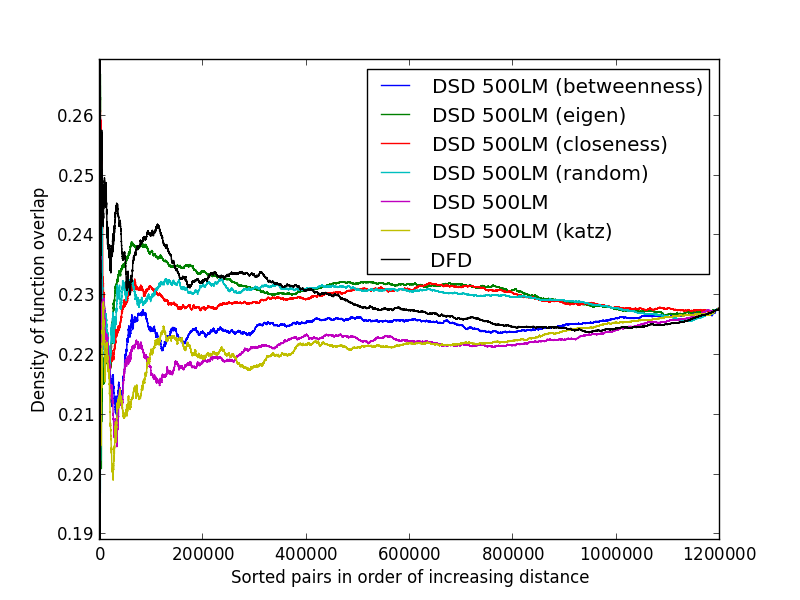
\includegraphics[width=0.333333333333\textwidth]{plots/landmark_comps/500LM/rat_alld_pairs_density.png}
}
\subfloat[Mouse]{
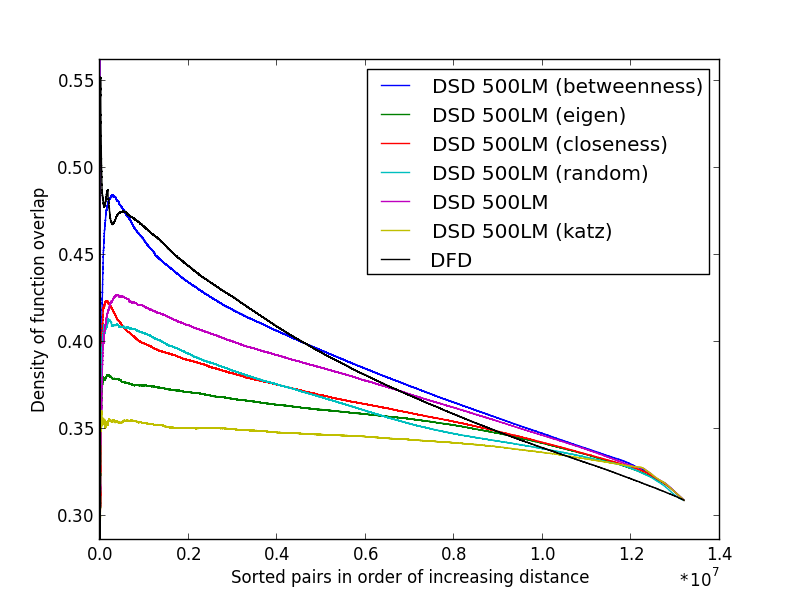
\includegraphics[width=0.333333333333\textwidth]{plots/landmark_comps/500LM/mouse_alld_pairs_density.png}
}
\subfloat[Worm]{
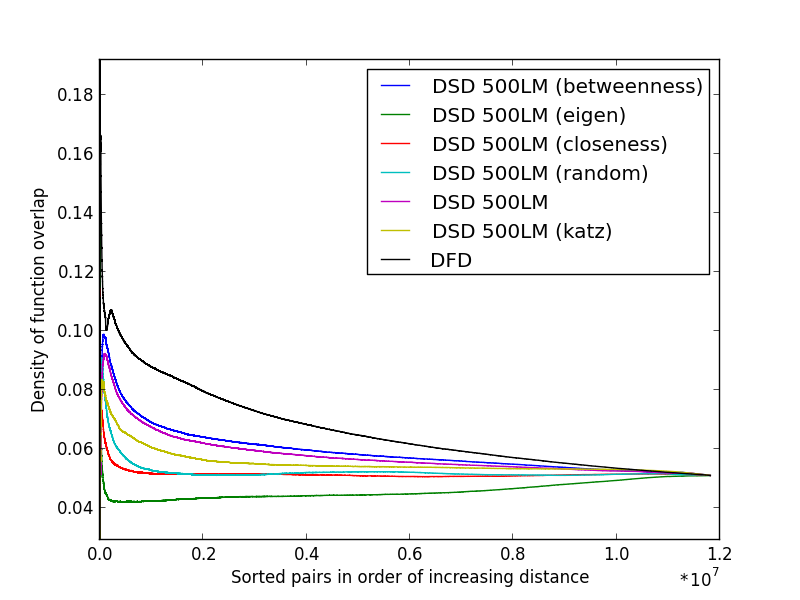
\includegraphics[width=0.333333333333\textwidth]{plots/landmark_comps/500LM/worm_alld_pairs_density.png}
}
}
\centerline{
\subfloat[Fly]{
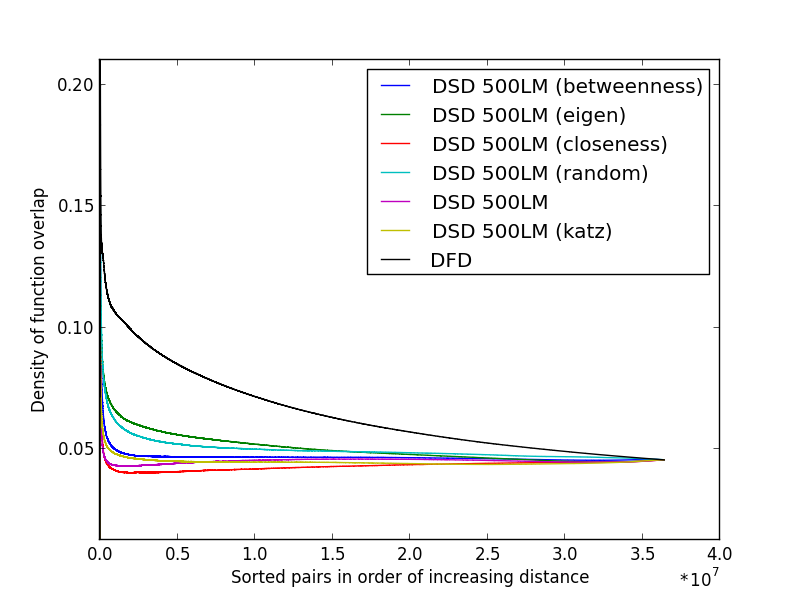
\includegraphics[width=0.333333333333\textwidth]{plots/landmark_comps/500LM/fly_alld_pairs_density.png}
}
\subfloat[Yeast]{
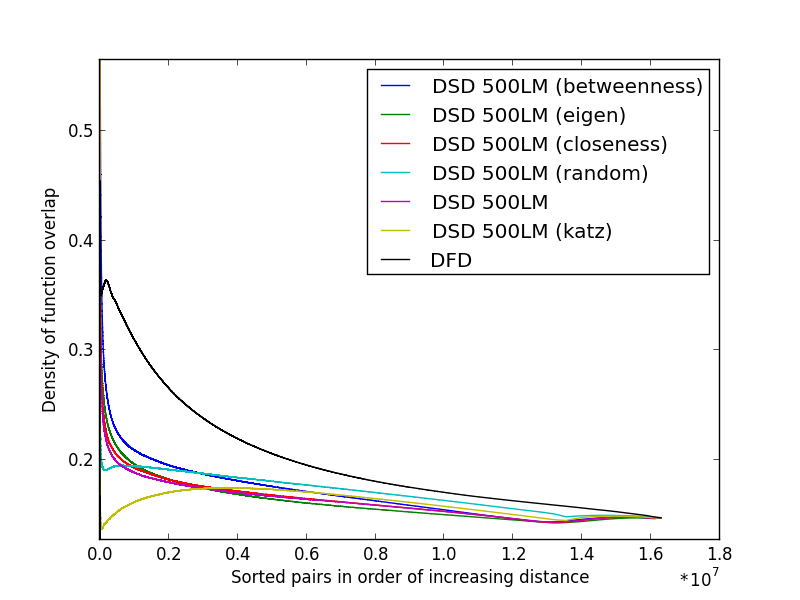
\includegraphics[width=0.333333333333\textwidth]{plots/landmark_comps/500LM/yeast_alld_pairs_density.png}
}
\subfloat[Human]{
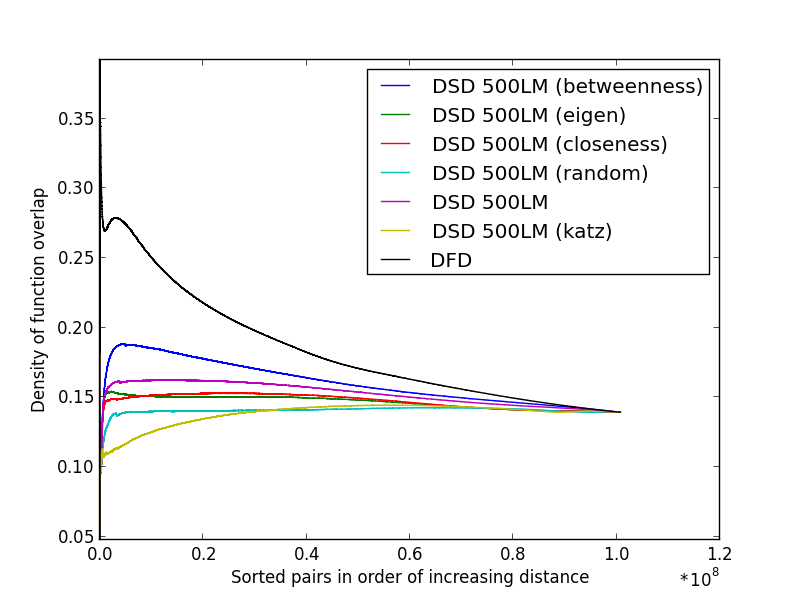
\includegraphics[width=0.333333333333\textwidth]{plots/landmark_comps/500LM/human_alld_pairs_density.png}
}
}
\end{figure}

\end{document}
